\chapter{システム}
本章では,日常生活動作別の時間記録アプリケーション,ADLoggerを提案する.
はじめにADLoggerシステムの概要を述べ,次にADLoggerの特徴を説明する.
そして最後に,ユーザがADLoggerを利用する流れについて述べる.

\section{ADLoggerシステムの概要}
ADLoggerはユーザの行動名別に経過時間を記録するiOSアプリケーションである.
ユーザは行動名毎に行動時間を実測で記録される.
予測算出画面では,行動別の平均時間がリスト形式でカラム毎に出力される.
カラムを複数選択する事で複数行動を行う際の必要時間を計算・可視化する事が可能である.

\section{ADLoggerシステムの特徴}
本節では,ADLoggerシステムの特徴としてあげられる機能を挙げる.
\subsection{タスク別ストップウォッチ記録}
内蔵されているストップウォッチで行動名毎に行動時間を実測で記録される.
\subsection{各時間予測}
各行動を下記の計算方法を用いてユーザの行動別記録時間の標準的な時間を算出し,リスト形式で行動別に表示する.
\subsection{合計時間の算出}
リストのカラムをタップすると,選択された行動の合計の必要時間を下記の計算手法を元に算出する.

\section{平均時間の算出方法}
\subsection{各時間予測}
行動別の時間の表示は前述した三点見積もり法を参考にした.
タスク完了に要する時間の期待時間を$TE$,記録内最短時間を$O$,記録内最長時間を$P$とすると,下記の様に見積もりを行う.
尚,先行研究の項目で述べた通り三点見積もり法の再確時間は通常最頻値を採用するが,今回は少ないデータ数でも見積もりが可能となる様代替として平均値を採用した.
\[ TE=\{ O + 4(\frac{1}{n}\displaystyle\sum_{i=1}^{n}x_{i}) + P\}/6\]

また,表には表示されないものの各タスクは三点見積もり法の標準偏差を求め,標準偏差の3倍をかける事で信頼範囲99.7\%の値を算出する.
\[ SD = (P - O)/2\]

\subsection{合計時間の算出}

先ほど算出したタスク毎の$T_{E}$と$SD$を用いて,ユーザが選択したタスクの合計時間$T_{sum}$を算出する.
数式は以下の通りとなる.
\[ T_{sum}= \displaystyle\sum_{i=1}^{n} (TE_{i} + SD_{i})\]
また標準偏差$SD$は,合計値の下に選択タスクの$SD$合計値$SD_{sum}$を「バッファ用時間」として算出する.
\[ SD_{sum}= \displaystyle\sum_{i=1}^{n}  SD_{i}\]
%これからきちんと書こう。秒単位で計測する分最頻値を出すのが時間がかかる為便宜的に他の手法を取った事も記述しよう。



\section{ADLoggerシステムの使用方法}
本アプリケーションを開くと,トップ画面が開かれる(図~\ref{fig:top}).
``LOGIN"ボタンを押すとユーザ名とパスワードが求められる(図~\ref{fig:login}).
初回の場合は下段の``REGISTERATION"ボタンから登録画面に移行し登録を行う(図~\ref{fig:reg}).
ログインが成功するとメイン画面に移行する(図~\ref{fig:ltop}).
尚,初回以降は直接メイン画面に移行する事が可能である.

メイン画面の``TIMER"ボタンにからは,行動を記録する事が可能である.
``TIMER"ボタンを押すと,``START"ボタンのあるストップウォッチ画面が現れる(図~\ref{fig:stopwatch}).
``START"ボタンを押すと``START"ボタンが``STOP"ボタンに切り替わった後,ストップウォッチが起動し時間を計測できる.
計測後は``STOP"ボタンを押す.出力されるアラートの中から``終了"ボタンを選択し,タスク名選択画面に移行する(図~\ref{fig:list}).
尚,記録を破棄したい場合はアラートの``Reset"ボタンを,ストップウォッチを止めたくない場合は`計測に戻る"を選択する.

タスク選択画面では行動名がリスト形式で表示されている.一度でも登録された行動名であれば行動名を選択する事で経過時間を保存する事ができる.
新たな行動名であれば``新規追加"ボタンを押し,出力されたアラートに行動名を入力し名前を登録後上記同様に保存する.

一度でも記録時間が保存されると``ADLog"ボタンから行動記録を閲覧する事が可能である(図~\ref{fig:log}).
ユーザは必要に応じてタスクを選択しする事で,複数タスクの合計時間を見る事が可能である.

利用規約,実験の説明,アプリの使用方法,設定などはトップ画面(図~\ref{fig:top})の``HELP"ボタンを押すと確認が可能な様にする(図~\ref{fig:help}).
後述する実験の関係上,ADLoggerボタンから行動記録の閲覧と,ストップウォッチスタート時のカウントアップの閲覧に関しては設定画面から制御できるようにした.

\begin{figure}[ht]
\begin{center}
\begin{tabular}{c}

	\begin{minipage}[b]{0.5\linewidth}
	\begin{center}
		\fbox{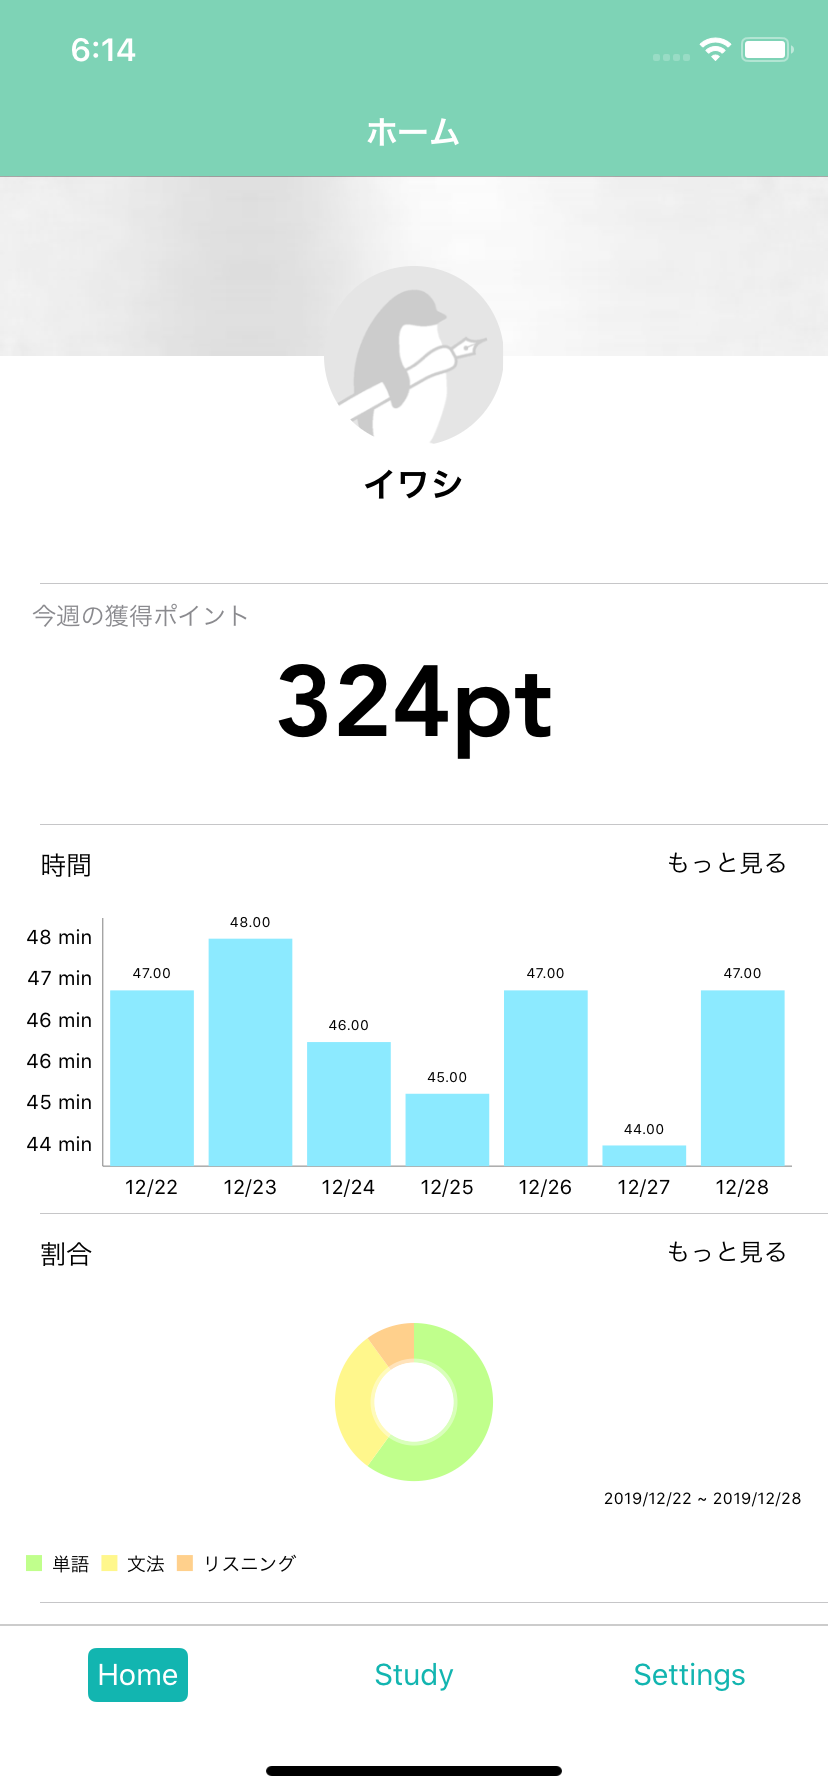
\includegraphics[width=5cm]{images/4/top.png}}
		\caption{トップ画面}
		\label{fig:top}
	\end{center}
  	\end{minipage}

	\begin{minipage}[b]{0.5\linewidth}
	\begin{center}
		\fbox{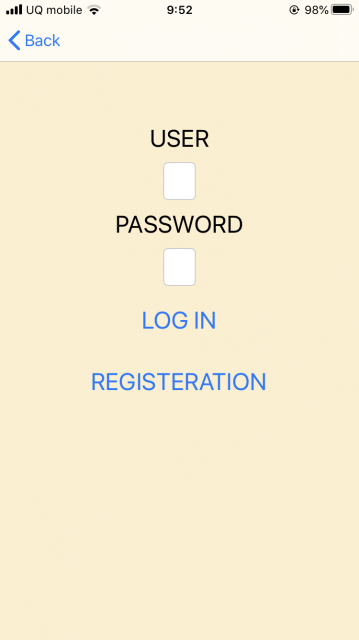
\includegraphics[width=5cm]{images/4/login.png}}
		\caption{ログイン画面}
		\label{fig:login}
	\end{center}
  	\end{minipage}
	
	\\
	
	\begin{minipage}[b]{0.5\linewidth}
	\begin{center}
		\fbox{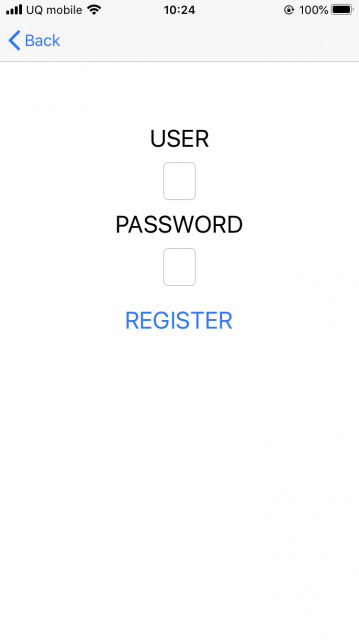
\includegraphics[width=5cm]{images/4/reg.png}}
		\caption{登録画面}
		\label{fig:reg}
	\end{center}
  	\end{minipage}
	
	\begin{minipage}[b]{0.5\linewidth}
	\begin{center}
		\fbox{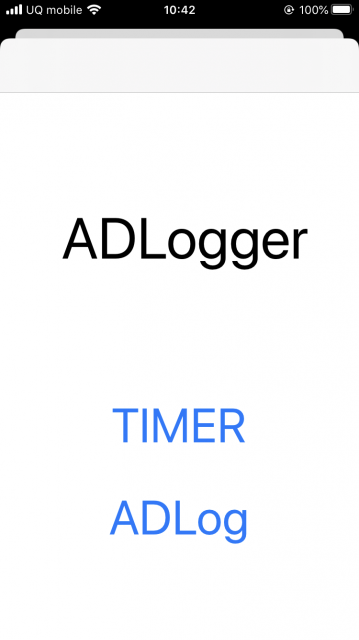
\includegraphics[width=5cm]{images/4/ltop.png}}
		\caption{メイン画面}
		\label{fig:ltop}
	\end{center}
  	\end{minipage}
	
  	\end{tabular}
  \end{center}
\end{figure}


\begin{figure}[ht]
\begin{center}
\begin{tabular}{c}

	\begin{minipage}[b]{0.5\linewidth}
	\begin{center}
		\fbox{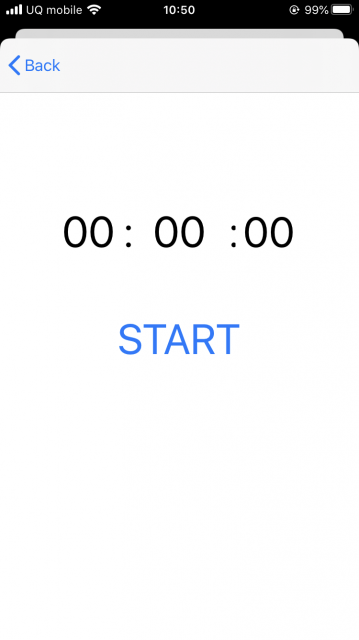
\includegraphics[width=5cm]{images/4/stopwatch.png}}
		\caption{ストップウォッチ画面}
		\label{fig:stopwatch}
	\end{center}
  	\end{minipage}
	
	\begin{minipage}[b]{0.5\linewidth}
	\begin{center}
		\fbox{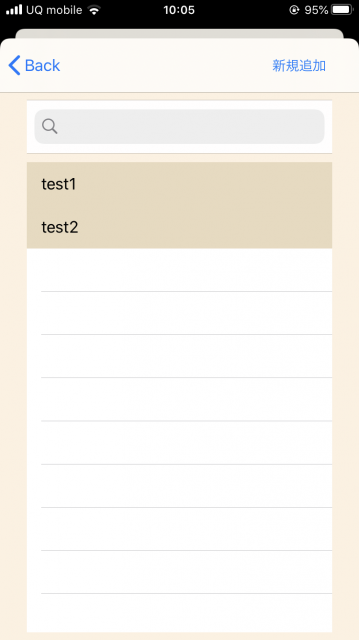
\includegraphics[width=5cm]{images/4/list.png}}
		\caption{タスク選択画面}
		\label{fig:list}
	\end{center}
  	\end{minipage}
	
	\\
	\begin{minipage}[b]{0.5\linewidth}
	\begin{center}
		\fbox{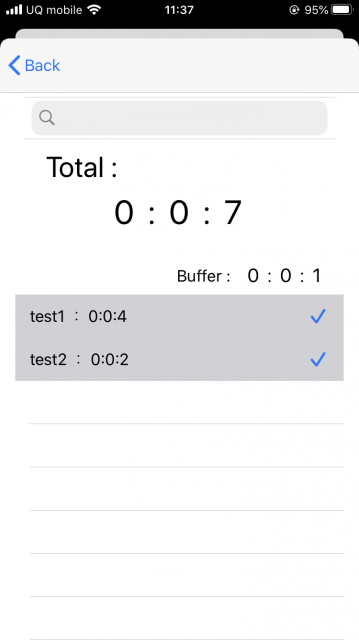
\includegraphics[width=5cm]{images/4/log.png}}
		\caption{ADLog画面}
		\label{fig:log}
	\end{center}
  	\end{minipage}
	
	\begin{minipage}[b]{0.5\linewidth}
	\begin{center}
		\fbox{
\includegraphics[width=5cm]{images/4/help.png}}
		\caption{HELP画面}
		\label{fig:help}
	\end{center}
  	\end{minipage}
	
  	\end{tabular}
  \end{center}
\end{figure}

\section{まとめ}
本章では,日常生活動作別行動時間記録及びリマインドを目的としたADLoggerシステムを提案した.
また,ADLoggerシステムの特徴および使用方法を述べた.
次章では,本システムの設計について述べる.